\begin{wrapfigure}[1]{r}[0cm]{4cm}
 \vspace{-6cm}
  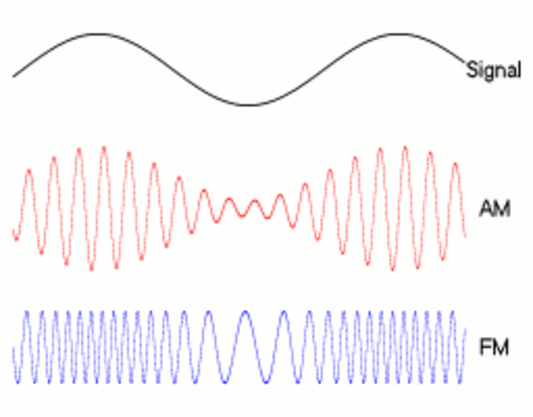
\includegraphics[scale=0.6]{Modulation/Bilder/Amfm3-en-de.pdf}
 \vspace{-6cm}
\end{wrapfigure}

\section*{Theorie- und Prüfungsfragen}

%~~~~~~

\subsection*{Sendearten}

\begin{enumerate} 
	\item[1] \emph{\textbf{BB401}}  Wie wird ``Morsetelegrafie, Zweiseitenband, ein einziger Kanal, der quantisierte oder digitale Information enthält, ohne Verwendung eines modulierten Hilfsträgers'', bezeichnet?
	\begin{enumerate}
	\itemsep1pt\parskip0pt\parsep0pt
		\item[A] NØN
		\item[B] A1A
		\item[C] A2A
		\item[D] R3E
		\loesung{Lösung B}
	\end{enumerate} 
	\item[2] \emph{\textbf{BB402}}  Wie wird ``Frequenzmodulation mit analogen Signalen, für Sprachübertragung'' bezeichnet?
	\begin{enumerate}
	\itemsep1pt\parskip0pt\parsep0pt
		\item[A] A3E
		\item[B] A2A
		\item[C] F3E
		\item[D] R3E
		\loesung{Lösung C}
	\end{enumerate} 
	\item[3] \emph{\textbf{BB403}}  Wie wird ``Einseitenbandmodulation mit analogen Signalen für Sprachübertragung'' (SSB) bezeichnet?
	\begin{enumerate}
	\itemsep1pt\parskip0pt\parsep0pt
		\item[A] J3E
		\item[B] J2E
		\item[C] R2A
		\item[D] A1A
		\loesung{Lösung A}
	\end{enumerate} 
\end{enumerate}

\subsection*{Modulationsarten}

\begin{enumerate} 
	\item[4] \emph{\textbf{TD501}}  Durch Modulation...
	\begin{enumerate}
	\itemsep1pt\parskip0pt\parsep0pt
		\item[A] werden Informationen auf einen oder mehreren Träger übertragen.
		\item[B] werden einem oder mehreren Trägern Informationen entnommen.
		\item[C] werden Sprach- und CW-Signal kombiniert.
		\item[D] werden dem Signal NF-Komponenten entnommen.
		\loesung{Lösung A}
	\end{enumerate} 
	\item[5] \emph{\textbf{TD502}}  Welche Aussage zur Frequenzmodulation ist richtig? Durch das Informationssignal
	\begin{enumerate}
	\itemsep1pt\parskip0pt\parsep0pt
		\item[A] wird die Amplitude des Trägers beeinflusst. Die Frequenz bleibt konstant.
		\item[B] werden die Frequenz und die Amplitude des Trägers beeinflusst.
		\item[C] findet keinerlei Beeinflussung von Trägerfrequenz oder Trägeramplitude statt. Die Information steuert nur die Kapazität des Oszillators.
		\item[D] wird die Frequenz des Trägers beeinflusst. Die Amplitude bleibt konstant.
		\loesung{Lösung D}
	\end{enumerate} 
	\item[6] \emph{\textbf{TB801}}  Was ist der Unterschied zwischen AM und SSB?
	\begin{enumerate}
	\itemsep1pt\parskip0pt\parsep0pt
		\item[A] AM hat einen Träger und zwei Seitenbänder, SSB arbeitet mit Trägerunterdrückung und einem Seitenband.
		\item[B] AM hat einen Träger und ein Seitenband, SSB arbeitet mit Trägerunterdrückung und hat zwei Seitenbänder.
		\item[C] AM hat keinen Träger und zwei Seitenbänder, SSB arbeitet mit Trägerunterdrückung und einem Seitenband.
		\item[D] AM hat keinen Träger und zwei Seitenbänder, SSB arbeitet mit Träger und einem Seitenband.
		\loesung{Lösung A}
	\end{enumerate} 
	\item[7] \emph{\textbf{TE102}}  Welches der nachfolgenden Modulationsverfahren hat die geringste Störanfälligkeit bei Funkanlagen in Kraftfahrzeugen?  
	\begin{enumerate}
	\itemsep1pt\parskip0pt\parsep0pt
		\item[A] SSB
		\item[B] DSB
		\item[C] AM 
		\item[D] FM
		\loesung{Lösung D}
	\end{enumerate} 
\end{enumerate}

\subsection*{Der Modulationsgrad}

\begin{enumerate} 
	\item[8] \emph{\textbf{TE103}}  Das folgende Oszillogramm (siehe Abbildung \ref{Modgrad} a) zeigt ein AM-Signal. Der Modulationsgrad beträgt hier zirka
	\begin{enumerate}
	\itemsep1pt\parskip0pt\parsep0pt
		\item[A] $67\%$
		\item[B] $33\%$
		\item[C] $50\%$
		\item[D] $75\%$
		\loesung{Lösung C}
	\end{enumerate} 
	\item[9] \emph{\textbf{TE105}}   Das folgende Oszillogramm (siehe Abbildung \ref{Modgrad} b) zeigt
	\begin{enumerate}
	\itemsep1pt\parskip0pt\parsep0pt
		\item[A] ein typisches Zweiton-SSB-Testsignal.
		\item[B] ein typisches Einton-FM-Testsignal.
		\item[C] ein typisches $100\%$-AM-Signal.
		\item[D] ein typisches CW-Signal.
		\loesung{Lösung A}
	\end{enumerate} 
	\item[10] \emph{\textbf{TE106}}   Das folgende Oszillogramm (siehe Abbildung \ref{Modgrad} b) zeigt[...]. Bestimmen Sie den Modulationsgrad
	\begin{enumerate}
	\itemsep1pt\parskip0pt\parsep0pt
		\item[A] Er beträgt $100\%$.
		\item[B] Er beträgt $0\%$.
		\item[C] Er beträgt ca. $50\%$.
		\item[D] Man kann keinen Modulationsgrad bestimmen, da es keinen Träger gibt.
		\loesung{Lösung D}
	\end{enumerate} 
\end{enumerate} 

\begin{figure}[H]
	\centering
	\subfigure[]{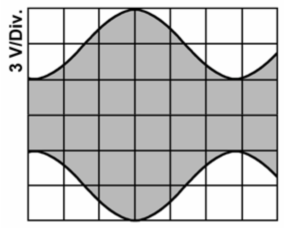
\includegraphics[scale=1]{Modulation/Bilder/Modulationsgrad.pdf}}
	\subfigure[]{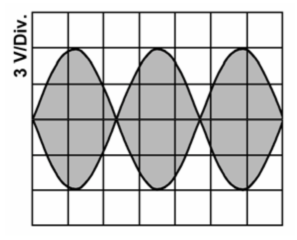
\includegraphics[scale=1]{Modulation/Bilder/Modulationsgrad2.pdf}}
	\caption{Modulationsgrad}
	\label{Modgrad}
\end{figure}